% Package

\documentclass[a4paper,10pt]{article}
\usepackage[utf8x]{inputenc}
\usepackage[T1]{fontenc}
\usepackage[francais]{babel}
\usepackage{graphicx}
\usepackage[export]{adjustbox}
\usepackage{listings}

% Include

\usepackage{listings}
\usepackage{color}

% Define Scala

\lstdefinelanguage{Scala}{
  morekeywords={abstract,case,catch,class,def,%
    do,else,extends,false,final,finally,%
    for,if,implicit,import,match,mixin,%
    new,null,object,override,package,%
    private,protected,requires,return,sealed,%
    super,this,throw,trait,true,try,%
    type,val,var,while,with,yield},
  otherkeywords={=>,<-,<\%,<:,>:,\#,@},
  sensitive=true,
  morecomment=[l]{//},
  morecomment=[n]{/*}{*/},
  morestring=[b]",
  morestring=[b]',
  morestring=[b]"""
}

\definecolor{dkgreen}{rgb}{0,0.6,0}
\definecolor{gray}{rgb}{0.5,0.5,0.5}
\definecolor{mauve}{rgb}{0.58,0,0.82}

\lstdefinestyle{Scala_style} {
	language=Scala,
  aboveskip=3mm,
  belowskip=3mm,
  showstringspaces=false,
  columns=flexible,
  basicstyle={\small\ttfamily},
  numbers=none,
  numberstyle=\tiny\color{gray},
  keywordstyle=\color{blue},
  commentstyle=\color{dkgreen},
  stringstyle=\color{mauve},
  breaklines=true,
  breakatwhitespace=true
  tabsize=3
}
\usepackage{listings}
\usepackage{color}

\definecolor{maroon}{rgb}{0.5,0,0}
\definecolor{darkgreen}{rgb}{0,0.5,0}


\lstdefinelanguage{XML_lang} {
  basicstyle=\ttfamily,
  morestring=[s]{"}{"},
  morecomment=[s]{?}{?},
  morecomment=[s]{!--}{--},
  commentstyle=\color{darkgreen},
  moredelim=[s][\color{black}]{>}{<},
  moredelim=[s][\color{red}]{\ }{=},
  stringstyle=\color{blue},
  identifierstyle=\color{maroon}
}

\lstdefinestyle{XML_style} {
	language=XML_lang,
	aboveskip=3mm,
  belowskip=3mm,
  showstringspaces=false,
  columns=flexible,
  breaklines=true,
  breakatwhitespace=true,
	tabsize=3
}

% Document

\begin{document}

% Flyleaf


\includegraphics[scale=0.1]{image/cristal.png}
\hfill

\includegraphics[scale=0.1]{image/lille1.png}

\vspace*{4cm}

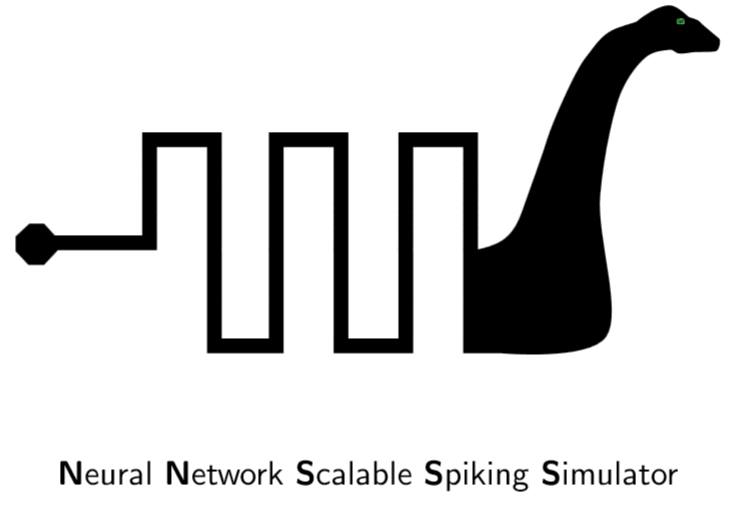
\includegraphics[scale=0.4]{image/n2s3.jpg}

\vfill
{\LARGE
\noindent
	Benjamin \textsc{Danglot}\newline
	Pierre \textsc{Falez}
}

\vfill
{
\noindent
{\LARGE Tuteur : Pierre Boulet} \hfill PJI 2015 
}

\newpage

% Table of contents

\tableofcontents

\newpage

% Introduction

\section*{Introduction}

\subsection*{Sujet} 
    Il s’agit du sujet 65 : \emph{Environnement de simulation d'un accélérateur neuromorphique}. Nous devions élaborer un langage dédié pour décrire un réseau de neurones ainsi qu’une simulation.

Mais le projet a eu d’autres besoins plus urgent, et nous avons donc développés les points importants que le simulateur avait besoin.

\subsection*{Motivations}
    Dans notre volonté de faire un doctorat, nous pensons que ce sujet était approprié pour nous apprendre des aspects de la recherche. De plus, l’utilisation de scala, et donc de son apprentissage était également un apport majeur à notre culture informatique. 
		
		Nous avons également pu découvrir une part de la bio-informatique ?? mb or not
% Project presentation

\newpage

\section{Présentation du projet}

\subsection{Technologies}

\subsubsection{Scala} 
\begin{figure}[h!]

\includegraphics[scale=0.15,right]{image/scala.png}
\end{figure}
\paragraph{}
Scala est un langage de programmation multi-paradigme crée par l’Ecole polytechnique fédéral de Lausanne (EPFL). Il combine la programmation orientés objet et le fonctionnel. Le langage Scala permet également de passer à l’échelle, et le fait qu’il utilise la machine virtuelle java (JVM) permet une portabilité sur différentes plateformes et ainsi l’utilisation de cluster pour fonctionner.

\subsubsection{Akka} 
\begin{figure}[h!]

\includegraphics[scale=0.1,right]{image/akka.png}
\end{figure}
\paragraph{}
Akka est une bibliothèque disponible en Java et Scala qui permet d’y ajouter de la concurrence et de la distribution, via un système d'acteur et de message.
        
\subsubsection{JspikeStack} 

\paragraph{}
JspikeStack est une application écrite en Java basée sur le modèle d'une machine de Boltzmann restreinte, qui construit et simule un réseau neuronal. Il permet notamment d’utiliser le réseau pré-appris Mnist, qui reconnaît les chiffres à partir de caméras.

\subsubsection{Memristor} 

\paragraph{}
Les memristors sont des composants électroniques dit passifs, il vient de la contraction de “memory” et “resistance”. Ce composant utilise sa résistance qui peut varier grâce à un courant électronique pour stocker de l’information. Le memristor a été “prédit” en 1971 par Leon Chua, mais aucun exemple physique n’a vu le jour avant 2008 par une équipe de chercheurs des laboratoires HP. Les memristors peuvent être vues comme des neurones, d’où l’implémentation d’un simulateur pour étudier le comportement de ces nouveaux composants.

\newpage

\subsection{État actuel}

\paragraph{}
Notre PJI est la suite directe d’un PJI de l’année dernière, ainsi que d’un projet M2. Nous avons donc put rencontrer les étudiants qui ont démarrés le projet, et ainsi avoir une présentation de leurs travaux.

\paragraph{}
Il s’agit de l’implémentation d’un simulateur de neurones à base de “Spike”, les messages que s’échangent les neurones grâce au synapses par lesquelles ils sont reliés. Il y a plusieurs simulateur déjà existant, mais qui  ont certains problèmes, notamment le passage a l’échelle, et donc une limitation dans les performances de simulation\footnote{par exemple BRIAN, développait en python. L'utilisation du python limite le nombre de neurone pouvant être utilisés}. Le projet est baptisé N2S3 (Nessie) : \emph{Neural Network Scalable Spiking Simulator}.

\paragraph{}
Lorsque que nous avons repris le projet, ce dernier avait déjà certaines fonctionnalités partiellement ou complètement opérationnelles.

\paragraph{}
Le projet à été pensée de façon générique : il doit pouvoir s’adapter a différent modèle de réseau. Pour le moment seul le modèle QBG est implémenté (expliquer qbg => tu sais ce que c’est toah? ?). C’est pourquoi le projet est répartie dans différents packages de la façon suivante : un package core contient les classes génériques pour représenter un réseau. un package feature.io pour toutes les fonctionnalités d’entrées/sorties, un package feature.logging pour la gestion des logs et enfin un package models.qbg pour implémenter un réseau de ce type.

\paragraph{}
L’implémentation du réseau à été pensée de la manière suivante : chaque neurone et chaque synapse est représenté par un acteur. A l’époque, un synchronizer, qui est également  un agent, était en charge de récupérer tous les messages, et de les redistribuer à travers le réseau pour que la cohérence dans le temps soit bien respectée. 

\paragraph{}
Les neurones sont réparties dans différentes couches. Comme le simulateur pour le moment suit le modèle restreint de machine de Boltzmann, les seules communications entre les neurones se font entre des couches voisines. Il n'y a donc pas non plus d’interconnexion entre des neurones d'une même couche.

\paragraph{}
Avec le modèle actuel, chaque neurone possède un potentiel qui, lorsqu'il dépasse un seuil fixé, va envoyer un spike à l'ensemble des neurones qui sont reliés avec lui. Chaque synapse possède un poids synaptique qui varie au cours de la simulation en fonction des spike qui affectent ou non le neurones dans une certaine fenêtre de temps. Pour reproduire ce comportement, différents types de spike ont été crée : 
\begin{itemize}
\item \emph{PreSynapticSpike} qui est le spike envoyé par les neurones vers une synapse
\item \emph{PostSynapticForwardSpike} qui est le spike envoyé par une synapse vers un neurone. Cette dernière transmet son propre poids synaptique au neurone.
\item \emph{PostSynapticBackwardSpike} qui est le spike renvoyé par le neurone vers ses synapses lorsque son potentiel a dépassé le seuil fixé. Celui-ci est nécessaire pour affecter le poids synaptique en fonction de la réaction du neurone.
\end{itemize}

\paragraph{}
Pour commencer la simulation, il suffisait de lancer des messages dans le réseau sur les neurones des premières couche afin de les stimuler.

\subsection{Perspectives du travail réalisés}
\paragraph{}
Le simulateur fonctionne globalement, mais certains aspects été a revoir :
\begin{itemize}
\item{La fourniture à la main d’entrées dans le simulateur n’est pas une solution convenable, de même que la création d’un réseau neuronale.}
\item{Les visualisations actuelles ne sont pas satifaisantes, et les logs ne permettent pas de bien comprendre l’évolution du réseau.}
\item{Avec un unique synchronizer pour le simulateur, le passage à l’échelle est impossible, il devient le goulot d’étranglement et ralentis toutes la progression de la simulation.}
\end{itemize}

\paragraph{}
Nous avons donc travaillé sur ces points, afin de permettre à N2S3 d’évoluer.

\newpage

\section{Ajout des Entrées}

\paragraph{}
Notre première tâche dans ce projet fût de mettre en place un système d'entrées afin de pouvoir stimuler le réseau. Celle-ci fût une bonne introduction pour nous, car elle nous a permit de prendre en main et d’aborder pas à pas le projet

\paragraph{}
Les fichiers JAER contiennent les données produites, par exemple, par une caméra à impulsion. Ce fichier se présente sous la forme d’une liste d'évènements. Chaque évènement étant représenté par un timestamp et une source. Ainsi, notre tuteur avait déjà implémenté une classe qui lit ces fichiers à partir d’une librairie ajoutée à N2S3. 

\paragraph{}
Pour gérer ces évènements d’entrées, nous avons créer une classe abstraite(cf InputGenerator.scala) dont l’implémentation dépendra du format de fichier d’entrée. Étant donnée que nous avions a notre disposition des fichiers JAER, et une classe de lecture, nous avons directement ajouter une classe pour ces formats de fichiers.

\paragraph{}
Cette classe se chargera de lire, et de placer d’en une file les évènements. Dans les premières versions, la gestion des entrées était totalement “indépendante” du réseau. Tant qu’il y avait des entrées, on les envoyés au synchronizer. Mais cette méthode le surchargeait, et donc ralentissait l’évolution du réseau. A présent, le synchronizer demande des entrées lorsqu’il juge qu’il en a besoin(un seuil, ou sa file est quasiment vide). Ce qui dynamise la simulation.

\newpage

\section{Création de réseau à partir de fichier XML}

\paragraph{}
Nous avons ensuite développé une classe qui permet de créer un réseau neuronale à partir d’un fichier XML.
Nous avons pris comme base, les fichiers XML utilisés par Peter O’Connor dans sa thèse (Annexe \ref{xml_exemple}). La classe permet d’initialiser le réseau, de connecté les neurones et les synapses ainsi que de leur affectés des potentiels/seuils à l’initialisation.

\paragraph{}
Ce fichier est construit de la manière suivante. L'ensemble du réseau est décrit à l'intérieur de la balise \emph{Network}. On retrouve notamment le nom du réseau, son type, le nombre de couche ainsi que des paramètres optionnels (température, fréquence de mise à jour, etc ...). Puis pour chaque couche, il y a une balise \emph{Layer} contenant la description de cette dernière. Chaque couche est identifié par un index, via la balise \emph{index}. Elle possède également une couche cible, \emph{targ}, qui est la couche de sortie avec laquelle ses neurones sont connecté. De plus, \emph{nUnits} donne le nombre de neurone contenue dans la couche courante et \emph{dimx} \emph{dimy} leurs répartition sur un plan à deux dimensions. Enfin, chaque seuil des neurones de la couche est représenté par un flottant simple précision encodé sous forme de base 64 dans la balise \emph{thresh} et de la même manière chaque poids synaptique est encodé dans la balise \emph{W}. Comme on travaille avec des modèle de machine de Boltzmann, les neurones entre deux couche voisine sont relié de façon complet : Chaque neurone possède une connexion vers l'ensemble des neurones de la couche voisine.

\paragraph{}
Pour réalisé cette fonctionnalité, nous avons utilisé la bibliothèque XML directement intégré à Scala. Nous récupérons dans un premier temps le nombre de couche et le nombre de neurones pour chaque couche ainsi que la topologie de ces dernières. A partir de ces informations, nous construisons et initialisons le réseau. Nous avons ensuite crée des message afin de pouvoir modifier les paramètres des neurones et des synapses (leurs seuil et leurs poids synaptiques). Enfin nous avons décodé ces paramètres pour chaque neurones et chaque synapses. (Annexe \ref{xml_builder})

\section{Amélioration du synchronizer}

\subsection{Génération d'entrée à la demande}
\subsection{}

\newpage

\section{Génération de graphes}

\paragraph{}
Nous avons mis en place une génération de graphe à partir des fichiers de log crée par chacun des acteurs. En effet, pour pouvoir apprécier les simulations et leurs résultats, une visualisation graphique est nécessaires.
Celle-ci s'effectue généralement en deux passes : 
\begin{itemize}
	\item{1}: La lecture du fichier de log et la création de variables qui permettent de configurer correctement les fichiers qui seront générés.
	\item{2}: La génération en elle-même, qui crée deux fichiers : un fichier de données contenant toutes les informations que le graphe a besoin pour répondre au besoin de l'utilisateur, et un fichier plot, qui utilise ce fichier de données et les variables définis durant la lecture.
\end{itemize}

\subsection{Graphes d’activité des neurones}
\paragraph{}
A partir des logs que les neurones créent, nous pouvons générer un graphe d’activité neuronales. 

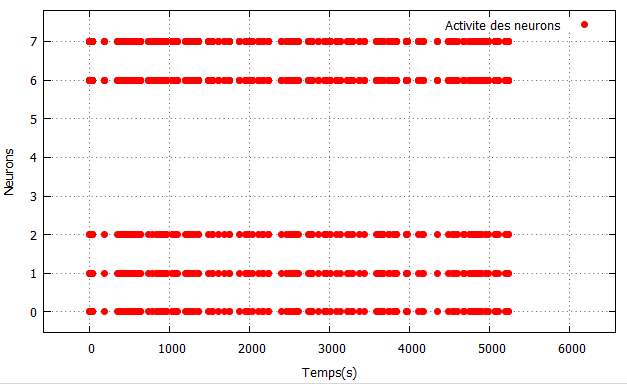
\includegraphics[scale=0.95,right]{image/neuronActivity.png}

\paragraph{}
Certaines options sont disponibles pour générer ce type de graphes :
\begin{itemize}
\item{Donner la liste des index des neurones que l’on souhaite observer.}
\item{Donner la liste des index des couches que l’on souhaite observer.}
\item{Donner un temps maximum.}
\end{itemize}

\subsection{Graphes des activités des synapses}

rubarberubarberubarberubarberubarberubarberubarberubarberubarbe

\subsection*{Remarques}
\paragraph{}
ces générations se font pour l’instant sur de petits exemples de fichiers de logs, mais il faut l’améliorer pour pouvoir visualiser sur de véritables simulations, avec des réseaux de l’ordre de millions de neurones.

\appendix
\section{Code samples}

\subsection{Gestion des entrées}
\subsection{Construction de réseau à partir d'xml}
\subsection{Génération de graphes}

Examples de code pour la génération de graphes de l'activité neuronales.
Boucles pour construire le fichier de données.
\lstinputlisting[language=scala,breaklines=true]{src/loopdata.scala}
Génération du fichier plot
\lstinputlisting[language=scala,breaklines=true]{src/pltgen.scala}

\section{Example de fichier xml}
\label{xml_exemple}

Voici l'exemple du fichier XML utilisé par Peter O'Connor dans sa thèse, sur lequel nous avons batis notre constructeur de réseau à partir de fichier XML :
 
\lstinputlisting[style=XML_style]{src/example.xml}

\section{Code du générateur de réseau via fichier XML}
\label{xml_builder}
\lstinputlisting[style=Scala_style]{src/XMLBuilder.scala}


\section{Example de fichier de graphe (gnuplot)}

Voici un exemple de fichier plot généré grâce à l'application, il concerne l'activité neuronale du réseau : 

\lstinputlisting[breaklines=true]{src/neurons.plt}


\end{document}